\chapter{Migration process}

This chapter describes the process of migrating a web application to serverless architecture. The goal of the migration is to explore the feasibility of the catalogued patterns by applying them on common problems in the domain of web application development. In cases where the patterns prove insufficient or unsuitable to the problem in hand, modifications or new patterns are proposed. As well as exploring the patterns we're seeing how the distinct serverless features drive application design and try to gain deeper understanding of the advantages and shortcomings of the paradigm. Finally in chapter \ref{cha:evaluation} the migration outcome is evaluated against the pre-migration application in terms of quality and ease of development.

The migrated application, Image Manager, is a tool for managing image assets. The application is adapted from a real-world work assignment, slightly modified for the sake of illustration. Similarly to a SaaS offering such as Cloudinary, the application takes user-uploaded images, does various forms of processing and then hosts and serves the processed images to be consumed by other applications. In case of Image Manager the processing needs are threefold: rendering a thumbnail, rendering a low quality image placeholder (LQIP), and automatic label detection. The two CPU-intensive rendering tasks are performed locally whereas labeling is offloaded to an external image analysis service, Google Cloud Vision API.

% We can thus roughly divide the application into four parts: API, authentication, image processing and image hosting.

Figure \ref{fig:serverfulArchitecture} presents the pre-migration serverful architecture. This implementation consists of a single server application that connects to a number of external services. The server application publishes a single API endpoint for image uploads which is consumed by a browser client. The public-facing API is protected with CAPTCHA-based authentication to prevent spam. The application is containerized into a Docker image and deployed on a single VM on Google Cloud Platform. The server application connects to a number of Google Cloud Platform services: processed images are stored on the object storage service Cloud Storage, image labeling is handled with the Vision API service, and the reCAPTCHA service is used for authentication. Figure \ref{fig:serverfulArchitecture} illustrates the image upload sequence in detail, showing how the various services fit together.

\begin{figure}[h]
  \centering
  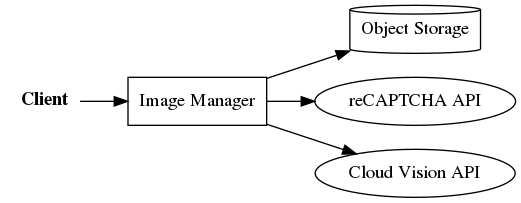
\includegraphics[width=0.65\textwidth]{image-manager.png}
  \caption{Serverful Image Manager architecture}
  \label{fig:serverfulArchitecture}
\end{figure}

\begin{figure}[h]
  \centering
  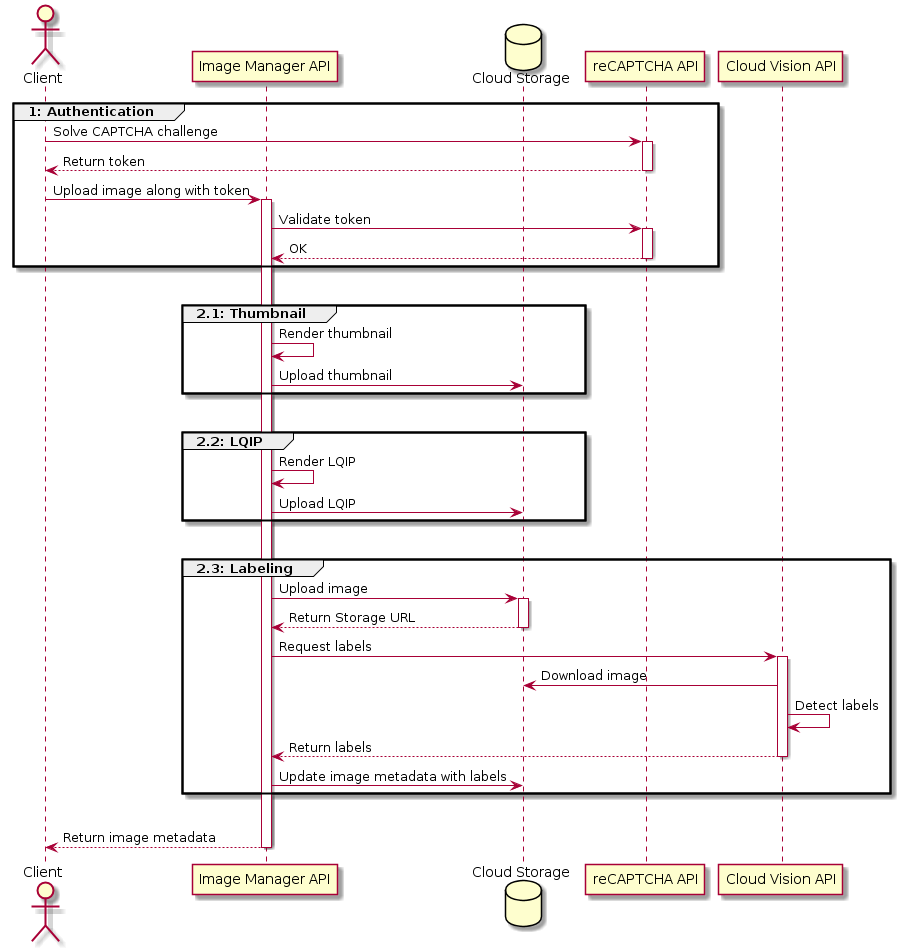
\includegraphics[width=0.85\textwidth]{sequence.png}
  \caption{Serverful Image Manager upload sequence}
  \label{fig:serverfulSequence}
\end{figure}

\ref{fig:serverlessArchitecture} presents the migrated serverless architecture, where the same functionality is split into separate serverless functions and tied together in an event-driven flow. In both figures rectangular boxes represent the parts that are implemented by hand, whereas the rest are external services. \ref{fig:serverlessSequence} illustrates the image upload sequence in our serverless implementation.

% TODO Building both deployment artifacts from the same code base. describe migration process step-by-step? API, authentication, processing and upload?

\begin{figure}[h]
  \centering
  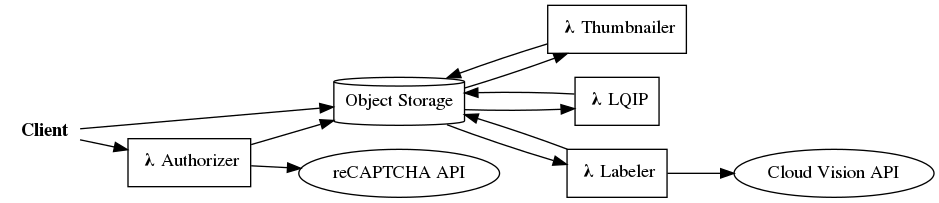
\includegraphics[width=\textwidth]{image-manager-serverless.png}
  \caption{Serverless Image Manager architecture}
  \label{fig:serverlessArchitecture}
\end{figure}

\begin{figure}[h]
  \centering
  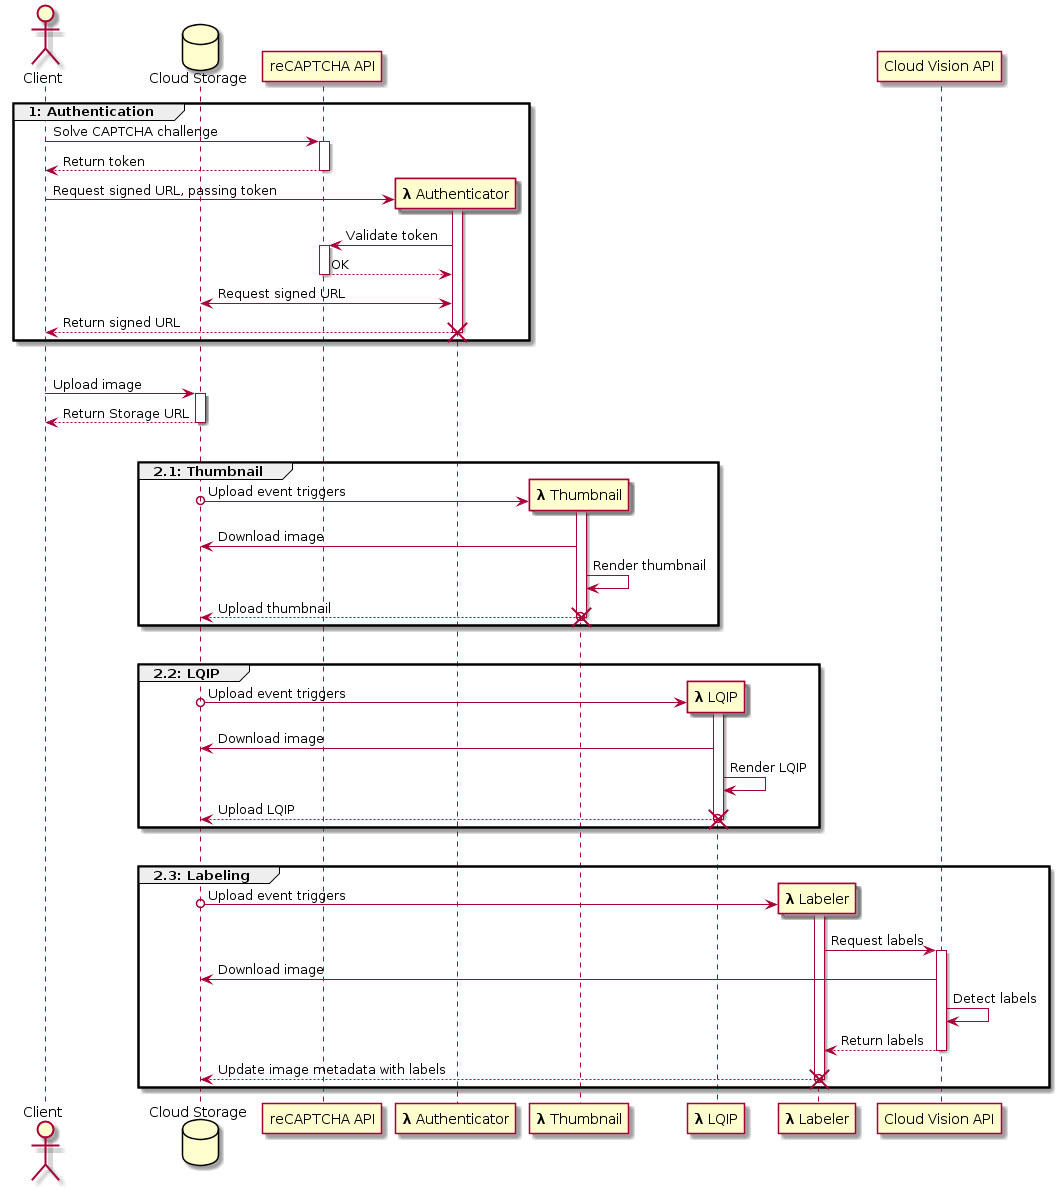
\includegraphics[width=0.85\textwidth]{sequence-serverless.png}
  \caption{Serverless Image Manager upload sequence}
  \label{fig:serverlessSequence}
\end{figure}

\section{New patterns} \label{sec:newPatterns}

Here are some patterns to address problems I came across while sketching out the above serverless implementation:

\subsection{Fetcher} \label{subsec:Fetcher}
% or Local Threader?

\textbf{Problem:} Scaling an IO-bound operation out to parallel function instances is inefficient since the instances compete of the same IO resources.

\textbf{Solution:} Use local threading inside a single function instance to efficiently scale out operations like network requests.

E.g. three parallel functions each making a network request, or three parallel functions invoked by cloud storage upload that start execution by downloading the image: is it more efficient to have one function download the image and then invoke/pass the image as argument to three processing functions?

\subsection{Asynchronous Response} \label{subsec:AsyncResponse}

\textbf{Problem:} The client doesn't get any feedback from the asynchronous tasks it triggers.

\textbf{Solution:} Use a pub/sub channel to send a message to the client at the end of the task.

\subsection{Task Manager} \label{subsec:taskManager}

\textbf{Problem:} The client, after triggering an asynchronous task, has no way of tracking task progress or cancelling it.

\textbf{Solution:} Make each function instance subscribe to a pub/sub channel in the beginning of its execution in order to listen to client commands.

The former is one-way pub/sub, in Task Manager the function also subscribes.

\subsection{Throttled Recursion} \label{subsec:throttledRecursion}

\textbf{Problem:} Recursive serverless functions can overwhelm downstream resources by scaling out quickly or result in an infinite loop.

\textbf{Solution:} Pass recursive invocations through a message queue in order to control recursion speed.
